\documentclass[border=3pt,tikz]{standalone}
% Shared look for every TikZ figure in these notes.
% Included by each standalone figure file; also keeps the figures consistent
% with the colours used in the PDF and on the website.

\usepackage{tikz}
\usepackage{pgfplots}
\pgfplotsset{compat=1.18}
\usetikzlibrary{arrows.meta, decorations.markings, decorations.pathmorphing,
                patterns, calc, positioning}
\usepackage{amsmath}

% Series colours are the three validated categorical slots also used by the
% interactive widgets, so a path drawn in the printed notes and the same path on
% the website are the same colour. They clear the colour-vision-deficiency and
% contrast checks as a set; every path is direct-labelled as well, so colour is
% never the only thing carrying identity.
\definecolor{duPurple}{HTML}{68246D}
\definecolor{duBlue}{HTML}{2A78D6}
\definecolor{duRed}{HTML}{EB6834}
\definecolor{duGreen}{HTML}{1BAF7A}
\definecolor{duGrey}{HTML}{6B6B6B}

\tikzset{
  axisline/.style   = {-{Stealth[length=3mm]}, line width=0.7pt, black},
  path1/.style      = {duBlue,   line width=1.1pt},
  path2/.style      = {duRed,    line width=1.1pt},
  path3/.style      = {duGreen,  line width=1.1pt},
  statedot/.style   = {circle, fill=black, inner sep=1.4pt},
  arrowhead/.style  = {decoration={markings,
                        mark=at position #1 with {\arrow{Stealth[length=2.6mm]}}},
                       postaction={decorate}},
  lbl/.style        = {font=\small},
  slbl/.style       = {font=\footnotesize, duGrey},
  workfill/.style   = {duPurple, opacity=0.16},
}

\usetikzlibrary{shapes.geometric, shapes.arrows}
\definecolor{hotres}{HTML}{D99694}
\definecolor{coldres}{HTML}{8EB4E3}
\definecolor{engine}{HTML}{BFBFBF}
\begin{document}
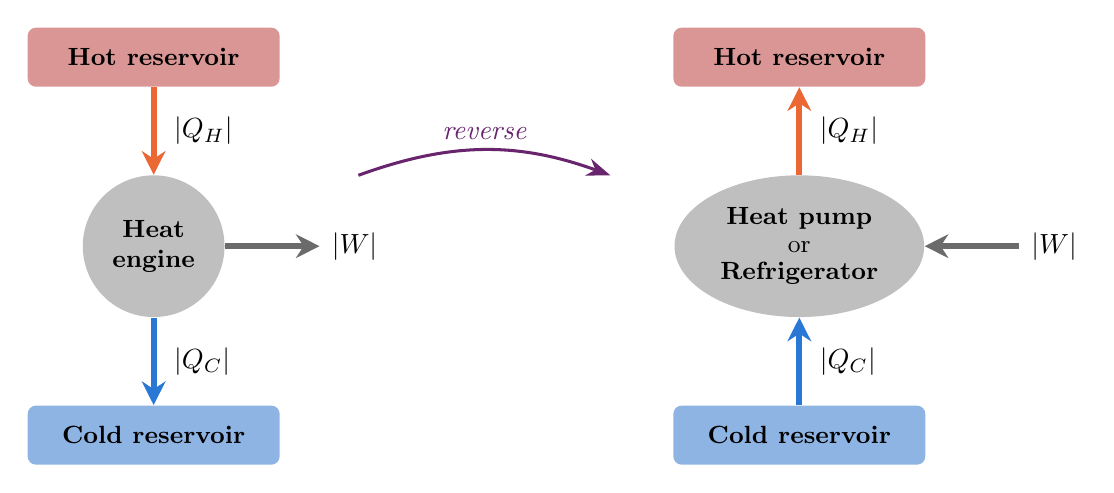
\begin{tikzpicture}[
  res/.style={rounded corners=3pt, minimum width=3.2cm, minimum height=0.75cm,
              font=\small\bfseries},
  flow/.style={-{Stealth[length=3mm,width=3mm]}, line width=2.2pt}]
  % reversible heat engine
  \begin{scope}
    \node[res, fill=hotres]  (H) at (0,2.4)  {Hot reservoir};
    \node[circle, fill=engine, minimum size=1.8cm, align=center,
          font=\small\bfseries] (E) at (0,0) {Heat\\engine};
    \node[res, fill=coldres] (C) at (0,-2.4) {Cold reservoir};
    \draw[flow, duRed]  (H.south) -- (E.north)
      node[midway, right=3pt, text=black] {$|Q_H|$};
    \draw[flow, duBlue] (E.south) -- (C.north)
      node[midway, right=3pt, text=black] {$|Q_C|$};
    \draw[flow, duGrey] (E.east) -- ++(1.2,0) node[right, text=black] {$|W|$};
  \end{scope}
  % reversed: refrigerator / heat pump
  \begin{scope}[xshift=8.2cm]
    \node[res, fill=hotres]  (H2) at (0,2.4)  {Hot reservoir};
    \node[ellipse, fill=engine, minimum width=2.8cm, minimum height=1.8cm,
          align=center, font=\small\bfseries] (E2) at (0,0)
          {Heat pump\\[-1pt]{\normalfont or}\\[-1pt]Refrigerator};
    \node[res, fill=coldres] (C2) at (0,-2.4) {Cold reservoir};
    \draw[flow, duRed]  (E2.north) -- (H2.south)
      node[midway, right=3pt, text=black] {$|Q_H|$};
    \draw[flow, duBlue] (C2.north) -- (E2.south)
      node[midway, right=3pt, text=black] {$|Q_C|$};
    \draw[flow, duGrey] ($(E2.east)+(1.2,0)$) -- (E2.east)
      node[pos=0, right, text=black] {$|W|$};
  \end{scope}
  \draw[-{Stealth[length=3mm]}, line width=1.1pt, duPurple]
    (2.6,0.9) to[bend left=20]
    node[midway, above, font=\normalsize\itshape] {reverse} (5.8,0.9);
\end{tikzpicture}
\end{document}
